%!TEX root = ../dissertation_vkslm.tex

\chapter{Proposed Method}\label{ch:method}


Although a simple static signature can be generated linking the points of the dynamic trajectory, additional dynamic information could be used to enrich the static signature. This addition is expected to lead more realistic and more discriminative images. Figure \ref{fig_approach} shows how the proposed approach is used to generate a static signature based on online data. 

In this chapter, we describe our proposed approach. First, the dataset used to train our model is described. Afterwards, we describe how the data was preprocessed. Finally, the CNN model is detailed. 

\begin{figure}[!htb]
\centering
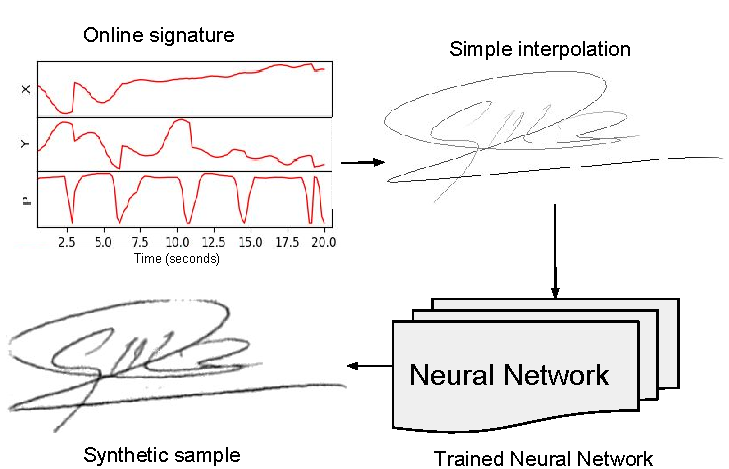
\includegraphics[width=0.8\textwidth]{method}
% where an .eps filename suffix will be assumed under latex, 
% and a .pdf suffix will be assumed for pdflatex; or what has been declared
% via \DeclareGraphicsExtensions.
\caption{The proposed approach diagram and an example of the synthetic signature generation.}
\label{fig_approach}
\end{figure}

\section{Online to offline training data}
In order to train our Neural Network to perform the approximation task of ``online to offline conversion'' we need both the online version of a handwritten manuscript containing the trajectory and pressure information mapped to the respective resulting offline representation, as in Figure \ref{fig:offon}. In order to acquire the online trajectory as well as the digital image for the same handwriting signal, some points have to be considered.

online signatures can't be projected in the respective offline version

don't match perfectly if you plot both in a single image (like your "onoff.png"). I'm not sure how they collected BiosecurID but this is a difficult problem to solve since BiosecurID was collected a long time ago in ATVS 

To the best of our knowledge the creators of the BiosecurID had not this characteristic in mind as well as the creators of other \cite{biomet, myidea, sigcomp2009, sigma, sigwicomp2013, sigwicomp2015} publicly available dual modal signature datasets.
\begin{figure}[!htb]
\centering
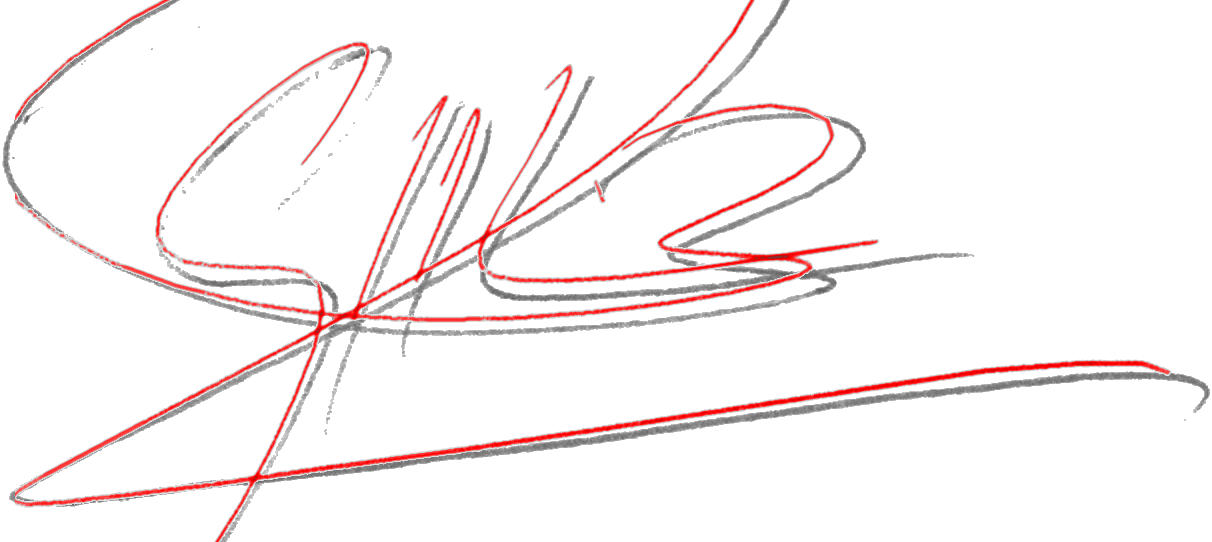
\includegraphics[width=0.5\textwidth]{onoff}
% where an .eps filename suffix will be assumed under latex, 
% and a .pdf suffix will be assumed for pdflatex; or what has been declared
% via \DeclareGraphicsExtensions.
\caption{The proposed approach diagram and an example of the synthetic signature generation.}
\label{fig:onoff}
\end{figure}


For each sample in the database, two complementary files are available. One of them, produced during the online acquisition, contains the list of the coordinates of the pen trajectory, the other one is the digital image of this piece of handwriting produced by the scanner. Of course, these two types of information should be available within the same coordinate system, with the same origin, the same resolution and orientation. But, as the two acquisition systems (tablet and scanner) are processing the writing separately and with their own parameters, this assumption is not satisfied directly. Geometrical transformations have to be applied to compensate for these differences.

The neural network was trained using the data from the IRONOFF dataset \cite{viard1999ireste}. The database contains a total of
23000 mapped online and
offline information of the handwriting manuscripts. The
offline handwriting signals have been sampled with a spatial
resolution of 300 dots per inch (DPI), with 8 bits per pixel
(256 gray level). The training data set contains 24,177 word
images, and another 12,219 images have been used as test
data.

\begin{figure}[!htb]
\centering

\includegraphics{ironoff-mapped}
% where an .eps filename suffix will be assumed under latex, 
% and a .pdf suffix will be assumed for pdflatex; or what has been declared
% via \DeclareGraphicsExtensions.
\caption{An offline manuscript mapped with the respective online trajectory. Image extracted from \cite{viard1999ireste}.}
\label{fig:ironoff-mapped}
\end{figure}


\section{Preprocessing}
%Copy and paste
The neural networks expect inputs of a fixed size, where signatures vary significantly in
shape (in IRONOFF, they range from small handwritten samples of size 167x214 to larger samples of size 548x215 pixels). In order to have a fixed size, we first normalize the images to the largest image size, by padding the images with
white background. In this case, we centered the manuscript in
a canvas of size 548x215 pixels, aligning the center of mass
of the sample to the center of the image, similar to previous
approaches in the literature, e.g. \cite{pourshahabi2009offline}. We then rescaled the
images to 383x150 pixels, i.e. 70\% of the canvas size, maintaining the aspect ratio of the original sample. This size was chosen to be large enough to keep
details from the pen strokes in the manuscript.

Besides resizing the images to a standard size, we also
performed the following pre-processing steps:
\begin{itemize}
\item Inverted the images: we inverted the images so that the white background corresponded to pixel intensity
0. 
\item Normalized the input: we normalized the input to the
neural network by dividing each pixel by the standard
deviation of all pixel intensities. We do not normalize the data to have mean 0 (another common pre-processing step) since we want the
background pixels to be zero-valued.
\item Interpolation: The online sequences ($x_{t}, y_{t}, p_{t}$) are linearly interpolated using the Bresenham line algorithm \cite{bresenham} to obtain 8-connected sequences.
\end{itemize}

Figure \ref{fig_ironoff} shows an example of the preprocessed input and the groundtruth that are being fed to the neural network during training phase.



\begin{figure}[!htpb]
\centering
 \subfloat[input]{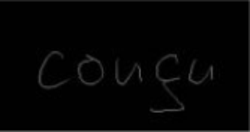
\includegraphics[width=2.0in]{input-ironoff}} 
\hspace*{0.5in} % separation between the subfigures
\subfloat[ground truth] {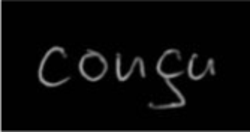
\includegraphics[width=2.0in]{gt-ironoff}}
\caption{Preprocessed data used during the training phase. (a) is the interpolated online sample, used as input and (b) is the expected prediction from the neural network, the ground truth. } \label{fig_ironoff}
\end{figure}



\section{Neural Network model}

The fully convolutional neural network (FCN) is adopted to learn an end-
to-end nonlinear mapping from online represetation to static image.

Our model is based on the concept of autoassociative memory \cite{jensen1996physiologically, weinberger2004specific}, commonly known as autoencoders. Autoencoders are normally used to reduce high-dimensional data into a low-dimensional code to later reconstruct the data from the compressed code, i.e., the desired output is the same of the input pattern \cite{kramer1991nonlinear, hinton2006reducing}. In our case, instead of expect the output to be the same as the input, our Neural Network model is fed with the interpolated online sample pressure information and we expect the respective offline sample on the output, i.e. the input is the pressure information and the desired output is the static manuscript.

\cite{springenberg2014striving}  we can remove each pooling layer and increase the stride of the convolutional layer that preceded it accordingly

We use an architecture based on the Convolutional Autoencoder \cite{masci2011stacked}. The expectation is that by learning to transform between online information to offline manuscripts, the network will learn convolution filters that are relevant to synthesize offline signatures based the online sample.


\begin{table}[!htb]
%% increase table row spacing, adjust to taste
\renewcommand{\arraystretch}{1.3}
% if using array.sty, it might be a good idea to tweak the value of
% \extrarowheight as needed to properly center the text within the cells
\caption{Summary of the CNN Layers}
\label{cnn-arch}
\centering
%% Some packages, such as MDW tools, offer better commands for making tables
%% than the plain LaTeX2e tabular which is used here.
\begin{tabular}{|l|l|}
\hline
\textbf{Layer}        & \textbf{Size} \\ \hline
Convolution           & 16x3x3        \\ \hline
Convolution           & 32x3x3        \\ \hline
Convolution           & 32x3x3        \\ \hline
Convolution           & 64x3x3        \\ \hline
Transpose Convolution & 64x3x3        \\ \hline
Transpose Convolution & 32x3x3        \\ \hline
Transpose Convolution & 32x3x3        \\ \hline
Transpose Convolution & 16x3x3        \\ \hline
\end{tabular}
\end{table}



We used the convolutions architecture similar to the one proposed on \cite{simonyan2014very} and the transposed convolutions were symmetric to the convolution operations. Some tests showed that the capacity of this network seems to be
too large for the problem at hand, particularly considering the
amount of convolution operations. We observed that the Neural Network was not learning useful transformations on the first few epochs. We obtained better results with. For the purpose of replicating our experiment, we provide a full list of the parameters used in our tests. Table \ref{table:cnn-arch} lists the definition of the Convolutional Autoencoder layers. For convolution and
transpose convolution layers, we list the size as NxHxW where N is the
number of filters, H is the height and W is the width of the
convolution and transpose convolution windows, respectively. 

We used Leaky Rectified Linear Units (LReLUs) the activation function for all convolutional layers. We also tried the Rectified Linear Units (ReLUs) but we observed that on the first 10 epochs the Neural Network seemed to be converging faster with the LReLUs. 

For every convolutional layer we use a stride (the distance between applications of the convolution operation) of 2x2, and we pad the input for every layer with 0  evenly left and right. We initialize the weights of the model using the technique proposed by Glorot and Bengio \cite{glorot2010understanding}, and the biases to 0. We trained the model with Adam optimizer to minimize the minimum squared error (MSE) loss for 100 epochs, using a learning rate of 0.001, and mini-batches of size 16. The network was trained using the library Tensorflow, and took around 72 hours to train on a GTX 670 GPU.

\section{Training Results}

\begin{figure}[!htb]
\centering
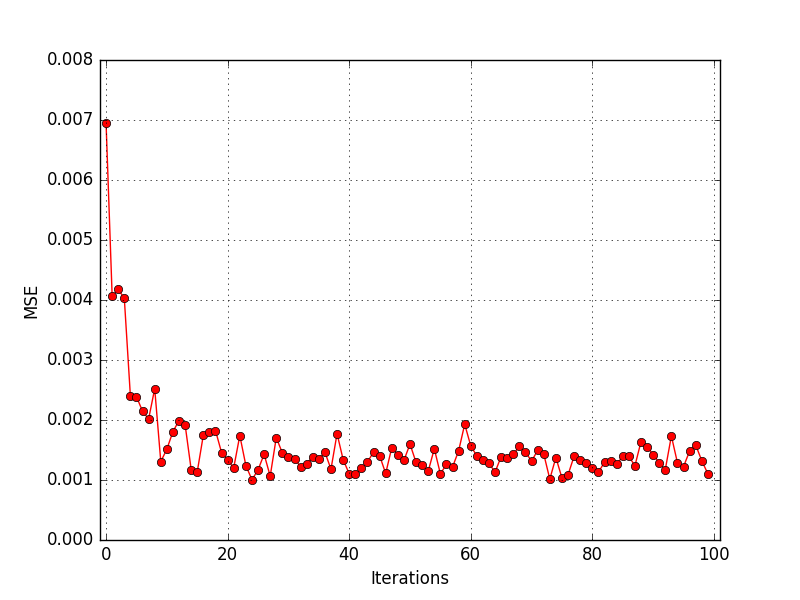
\includegraphics[width=5.5in]{iterations}
% where an .eps filename suffix will be assumed under latex, 
% and a .pdf suffix will be assumed for pdflatex; or what has been declared
% via \DeclareGraphicsExtensions.
\caption{Iterations versus MSE}
\label{fig:trainingMSE}

\end{figure}

\begin{figure}[!htpb]
\centering
\subfloat{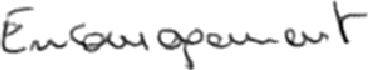
\includegraphics[scale=0.5]{samples/0}} 
\hspace*{0.4in} % separation between the subfigures
\subfloat{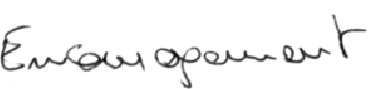
\includegraphics[scale=0.5]{samples/00}}
\\
\subfloat{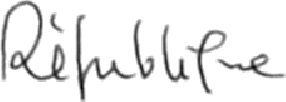
\includegraphics[scale=0.5]{samples/4}} 
\hspace*{0.4in} % separation between the subfigures
\subfloat{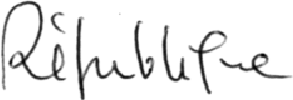
\includegraphics[scale=0.5]{samples/04}}
\\
\subfloat{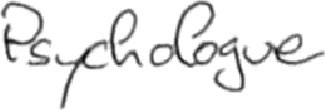
\includegraphics[scale=0.5]{samples/10}} 
\hspace*{0.4in} % separation between the subfigures
\subfloat{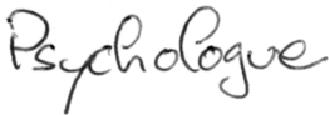
\includegraphics[scale=0.5]{samples/010}}
\\
\subfloat{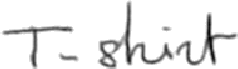
\includegraphics[scale=0.5]{samples/23}} 
\hspace*{0.4in} % separation between the subfigures
\subfloat{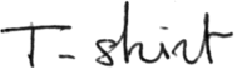
\includegraphics[scale=0.5]{samples/023}}
\\
\addtocounter{subfigure}{-8}
\subfloat[Synthetic Handwritten Manuscript]{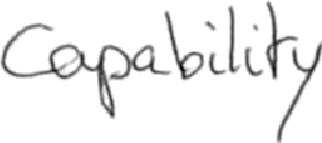
\includegraphics[scale=0.5]{samples/30}}
\hspace*{0.4in} % separation between the subfigures
\subfloat[Expected Real Manuscript - Groundtruth]{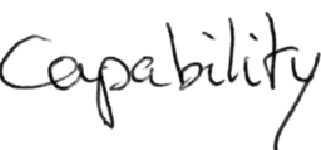
\includegraphics[scale=0.5]{samples/030}} 




\caption{Not cherry-picked} \label{fig:resultingsamples}
\end{figure}

